\section{Software Architecture}
This chapter describes the solution developed during our work. At the beginning the software architecture will be explained, followed by the partial steps and experiments which were needed to find the solution.
\\\\
The software architecture has to fulfil multiple requirements for this project. It should be easily extendable with new algorithms and ui extensions. The input and output format of the application should be independent from the algorithms to support different file types like bitmap images or \gls{gloss:DXF}/\gls{gloss:DWG} formats. The algorithms of the application should be link together as workflows which then can be executed by an engine in parallel.

\begin{figure}[h]
  \centering
      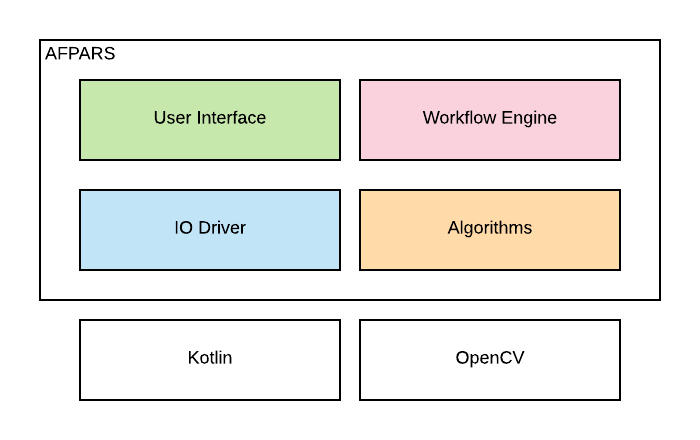
\includegraphics[width=0.8\textwidth]{AFPARS_Architecture}
  \caption{AFPARS software architecture.}
  \label{fig:AFPARS_Architecture}
\end{figure}

To fulfil these requirements, the architecture of the software is split into four parts as shown in Figure \ref{fig:AFPARS_Architecture}. The complete application is based on the \acrfull{acro:JVM} where \gls{gloss:Kotlin} is running on. For image processing and recognition the application uses the library \gls{gloss:OpenCV}.

\pagebreak

\subsection{Input / Output}
To support the different input and output formats the architecture uses a meta format for the
floor plan images called AFImage. Different drivers add the support for multiple file formats. With this architecture it is possible to extend the software with new file formats and work internally with the meta container.

\begin{figure}[h]
  \centering
      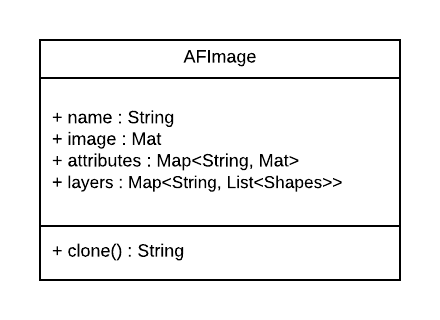
\includegraphics[width=0.5\textwidth]{AFImage_CD}
  \caption{AFImage class diagram.}
  \label{fig:AFImage_CD}
\end{figure}

The meta container AFImage contains multiple attributes (see Figure \ref{fig:AFImage_CD}) which can be used by algorithms to get information created by other algorithms or store information into an existing image.

\subsection{Algorithm}
blas

\begin{figure}[h]
  \centering
      \includegraphics[width=1\textwidth]{IAlgorithm_CD}
  \caption{Algorithm interface class diagram.}
  \label{fig:IAlgorithm_CD}
\end{figure}

bla

\subsection{Workflow}

\subsection{User Interface}
\missingfigure{User Interface Image.}
\todo{Why it looks like that. (Andere Software)}